\documentclass[a4paper, 11pt, final, garamond]{book}
\usepackage{cours-preambule}
\usepackage{pdfpages}

\raggedbottom

\makeatletter
\renewcommand{\@chapapp}{Travaux pratiques -- TP}
\makeatother

\let\SavedIndent\indent
\protected\def\indent{%
  \begingroup
    \parindent=\the\parindent
    \SavedIndent
  \endgroup
}
\setlength{\parindent}{0pt}

\begin{document}
\setcounter{chapter}{18}

\chapter{Mesure du coefficient adiabatique $\g$ de l'air par l'\'etude d'un
syst\`eme r\'esonant}

\section{Objectifs}

\begin{itemize}
    \item Observer des résonances d'amplitude pour un système mécanique.
    \item Déterminer la valeur numérique du coefficient adiabatique $\g$ de
        l'air par étude de sa compressibilité.
\end{itemize}

\section{S'approprier}
\subsection{Principe des mesures}

\begin{minipage}{0.56\linewidth}
    On considère un tube en verre horizontal dont une des extrémités est fermée
    et l'autre est en communication avec l'air ambiant. À l'intérieur de ce
    tube, un piston muni d'un aimant permanent peut se déplacer sans
    frottements. La bobine parcourue par un courant crée un champ magnétique
    sinusoïdal et excite l'aimant permanent qui se trouve à l'intérieur du
    piston. \bigbreak
    En faisant varier la fréquence du courant dans la bobine, on recherche la
    résonance en amplitude du piston. La fréquence de résonance est liée au
    coefficient adiabatique $\g$ de l'air que l'on se propose de déterminer.
\end{minipage}
\hfill
\begin{minipage}{0.40\linewidth}
    \begin{center}
        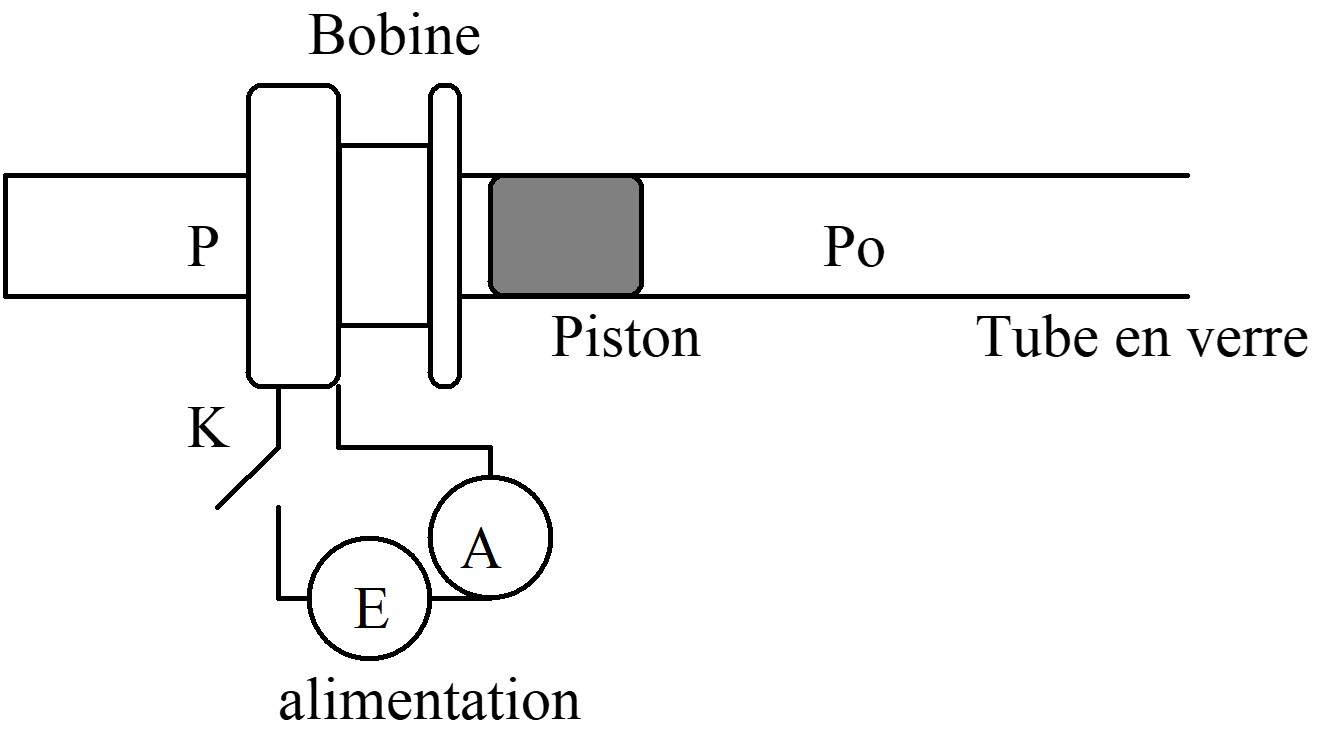
\includegraphics[width=\linewidth]{gamma1}
    \end{center}
\end{minipage}

\subsection{Étude mécanique du piston}
\begin{minipage}{0.56\linewidth}
    On étudie le système \{piston\} dans le référentiel du laboratoire, supposé
    galiléen. Il est soumis aux forces de pression qui s'exercent sur ses deux
    faces latérales, ainsi qu'à son poids et à la réaction du support, forces
    qui se compensent. Enfin, il est soumis à la force d'excitation magnétique
    $\vect{F}\ind{mag}$ engendrée par la bobine. On suppose cette force
    proportionnelle au courant $i(t)$ circulant dans la bobine selon
    \[
        \Ff\ind{mag} = \beta i(t) \ux
    \]
    avec $\beta$ une constante que l'on ne cherchera pas à déterminer. 
\end{minipage}
\hfill
\begin{minipage}{0.40\linewidth}
    \begin{center}
        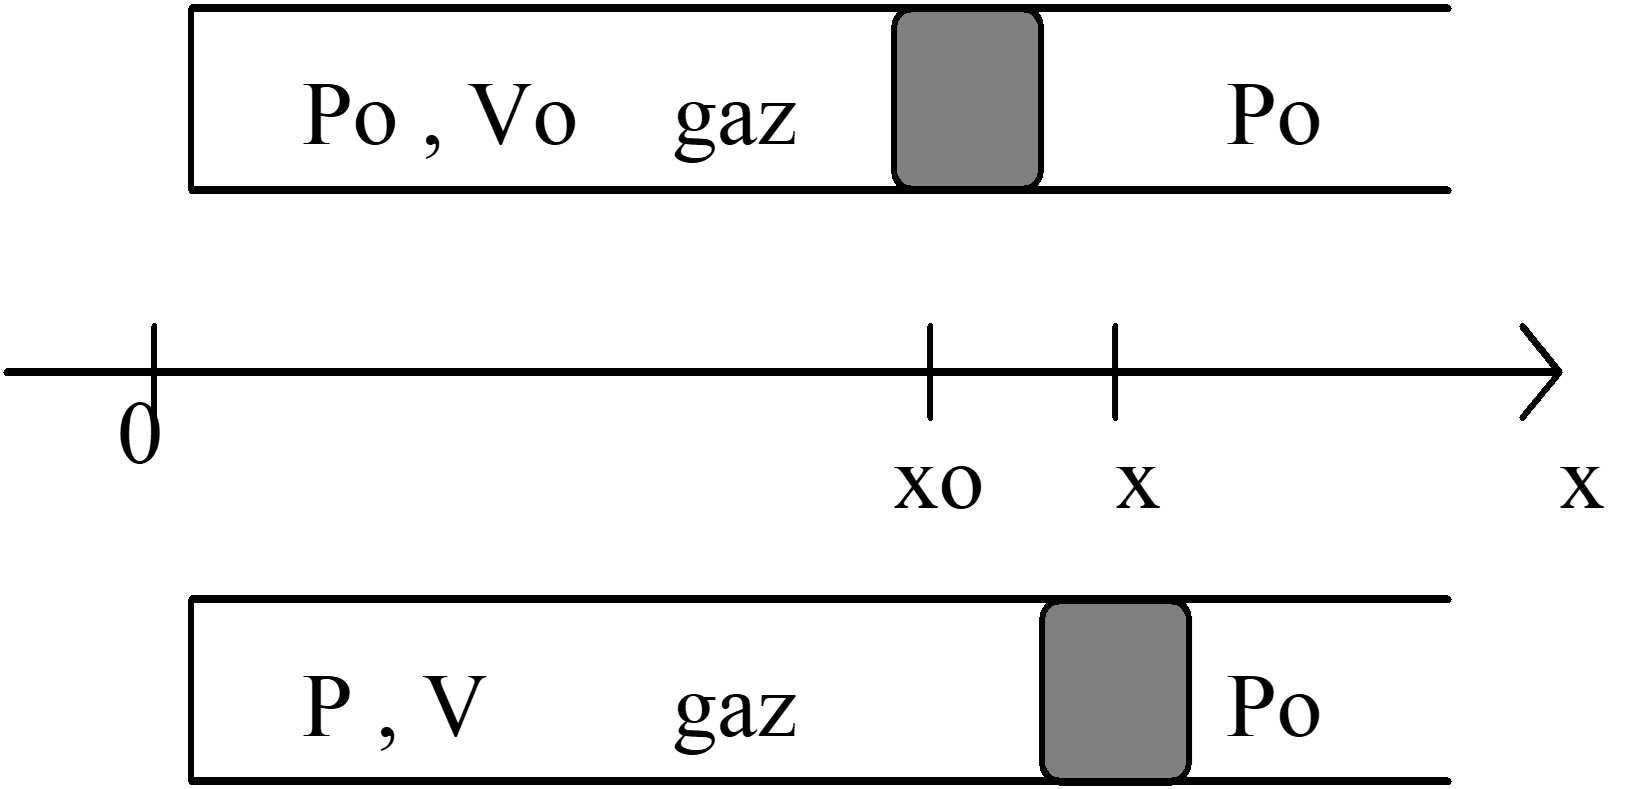
\includegraphics[width=\linewidth]{gamma2}
    \end{center}
\end{minipage} \bigbreak
Étudions le mouvement du piston selon l'axe horizontal $(Ox)$. À l'équilibre, le
piston se trouve en $x_0$, la pression étant égale à la pression atmosphérique
$P_0$ sur chaque face. Le volume fermé de gaz est $V_0$. On considère un petit
déplacement du piston dans le sens des $x$ croissants. Le volume de gaz fermé
devient $V$, et la pression qui s'exerce sur la face gauche du piston est $P <
P_0$ puisque le volume fermé de gaz a subi une détente. En appliquant la
deuxième loi de Newton en projection selon l'axe $(Ox)$, on obtient~:
\[
    \boxed{m\xpp = (P-P_0)S + \beta i(t)}
\]
où $m$ est la masse du piston et $S$ sa section.

\subsection{Transformations thermodynamiques subies par le volume fermé de gaz}

Au cours de l'expérience, les oscillations du piston sont suffisamment rapides
pour pouvoir supposer que les transformations subies par le gaz sont
adiabatiques, c'est-à-dire sans échange de chaleur avec l'extérieur. D'autre
part on assimile le gaz (l'air) à un gaz parfait de coefficient adiabatique $\g$
constant. Au cours de telles transformations, l'équation d'état du gaz suit la
loi dite de \textsc{Laplace} telle que
\[
    PV^\g = C
\]
avec $C$ une constante. L'expression différentielle de cette loi est~:
\[
    \frac{\dd P}{P} + \g \frac{\dd V}{V} = 0
\]
On en déduit donc une relation entre la variation de pression $\dd P$ du gaz et
sa variation $\dd V$ de volume au cours de la transformation.

\section{Analyser}
\subsection{Équation différentielle du mouvement}

D'après les caractéristiques du tube, $\dd V=S \dd x$. On suppose toutes les
variations faibles par rapport aux grandeurs de repos, si bien que
\[
    P = P_0 +\dd P \approx P_0 \qqet V = V_0 +\dd V \approx V_0
\]
Sous ces hypothèses, l'expression différentielle de la loi de \textsc{Laplace}
permet d'écrire~:
\[
    \dd P = -\g P_0 \frac{\dd V}{V_0}
\]
Et, en utilisant le fait que $\dd V = S \dd x = S (x-x_0)$,
\[
    \boxed{P-P_0 = \dd P = - \g \frac{P_0}{V_0} \, S \, (x-x_0)}
\]

\begin{enumerate}[label=\clenumi]
    \item Donner alors l'équation différentielle du mouvement du piston en $x$
    \item Vérifier que la pulsation propre du mouvement est
        \[
            {\w_0}^2 = \frac{P_0S^2\g}{mV_0}
        \]
    \item Montrer que le tracé de la \textbf{fréquence} de résonance au carré en
        fonction de $1/V_0$ est une droite de coefficient directeur $a$ dont on
        précisera l'expression.
\end{enumerate}

\subsection{Excitation de l'oscillateur}

Les frottements étant suffisamment faibles, le facteur de qualité est alors
grand devant 1, si bien que la pulsation de résonance obtenue expérimentalement
est très proche de la pulsation propre $\w_0$. On a donc accès expérimentalement
à la valeur de la fréquence propre du piston.

\section{Réaliser}
\subsection{Schéma du montage et alimentation de la bobine}
\begin{minipage}{0.56\linewidth}
    On alimente la bobine à l'aide d'un GBF sur sa \textbf{sortie amplifiée}
    $\SI{0,5}{\Omega}$), qui peut délivrer environ $\SI{1}{A}$ (nécessaire au
    fonctionnement du dispositif), ce qui est impossible avec la sortie
    classique du GBF. \bigbreak
    L'ampèremètre branché en série permet de vérifier l'intensité efficace
    débitée dans le circuit. Il faut qu'elle soit de l'ordre de
    \SIrange{0.8}{0.9}{A}, et toujours inférieure à $\SI{1}{A}$.
\end{minipage}
\hfill
\begin{minipage}{0.40\linewidth}
    \begin{center}
        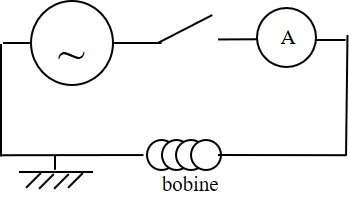
\includegraphics[width=\linewidth]{gamma3}
    \end{center}
\end{minipage}

\begin{minipage}{0.45\linewidth}
    On rappelle que la valeur efficace $S\ind{eff}$ d'un signal $s(t)$ dit
    $T$-périodique est définie par
    \[
        S\ind{eff} = \frac{1}{T} \sqrt{\int_{0}^{T} s^2(t)\dd t}
    \]
\end{minipage}
\hfill
\begin{minipage}{0.45\linewidth}
    Pour un signal sinusoïdal comme le courant ici, la valeur efficace est liée
    à l'amplitude $S_0$ selon~:
    \[
        S\ind{eff} = \frac{S_0}{\sqrt{2}}
    \]
\end{minipage}

\subsection{Mode opératoire}
Aller sur \texttt{Capytale}, en cliquant sur
\url{https://capytale2.ac-paris.fr/web/c/4523-1426759}
\begin{enumerate}
    \item Ouvrir le robinet de la burette, et choisir un volume initial $V_0$
        grâce à l'aimant. Notez cette valeur de $V_0$ dans la liste
        \texttt{python} correspondante, et fermer le robinet.
    \item Disposer alors la bobine de manière à ce que son bord se trouve à
        hauteur du bord du piston.
    \item Allumer le GBF et augmenter le \texttt{level} jusqu'à ce que
        l'intensité (lue sur l'ampèremètre) soit d'environ
        \SIrange{0.8}{0.9}{A}.
    \item Chercher la fréquence de résonance, en partant d'une fréquence de
        $\SIrange{40}{50}{Hz}$ environ et en la diminuant (ne pas descendre sous
        les $\SI{10}{Hz}$). À la résonance, le cylindre oscille alors avec une
        relativement grande amplitude.
    \item Noter cette valeur dans la liste \texttt{python} correspondante.
        Remplir la liste \texttt{Df0} de la plage de valeurs où vous estimez que
        la résonance se trouve (i.e.\ on a $f_0$ dans $[f_0 -\D, f_0 +\D]$)~;
        l'incertitude-type $u(f_0)$ est alors $\D/\sqrt{3}$.
    \item Ouvrir l'interrupteur pour couper le courant et lire le volume
        correspondant après oscillation. La différence avec $V_0$ correspond à
        l'écart à rentrer dans \texttt{DV0}, et l'incertitude-type sera alors
        \texttt{uV0 = DV0/np.sqrt(3)}.
    \item Déplacer de nouveau le piston en ayant ouvert le robinet, et faire
        ainsi une série de mesures en faisant varier $V_0$ et en repérant la
        valeur de $f_0$, sa plage d'existence et la plage d'existence de $V_0$
        pour chaque valeur de $V_0$.
\end{enumerate}

\section{Valider et conclure}

\begin{enumerate}[label=\sqenumi, start=4]
    \item Toujours sur \texttt{Capytale}, remplissez les listes des erreurs
        \textbf{relatives} pour $V_0$ et $f_0$ (l'incertitude divisée par la
        valeur).
    \item Créer les variables nécessaires au tracé de ${f_0}^2$ en fonction de
        $1/V_0$.
    \item Effectuer la régression linéaire avec \texttt{polyfit}, compléter la
        fonction définissant la régression linéaire, et tracer le graphique des
        données relevées avec la régression. Les erreurs à afficher sont les
        incertitudes absolues, pas relatives.
    \item La régression est-elle valide~?
    \item Relever le coefficient directeur $a$ de la droite modélisée. Quelle
        est son unité~?
    \item Déduire, de la partie Analyse, l'expression littérale du coefficient
        adiabatique $\g$ de l'air en fonction du coefficient directeur $a$ de la
        droite modélisée, de la masse $m$ de l'aimant, \textbf{du diamètre $d$
        du piston} et de la pression atmosphérique $P_0$.
    \item On a $m = \SI{8,8}{g}$ et $d = \SI{13,97}{mm}$. La pression
        atmosphérique $P_0$ se lit sur le baromètre placé dans la salle (en
        \si{mbar}). Après avoir détaillé les valeurs expérimentales et leurs
        unités correctes sur votre copie, utilisez \texttt{Capytale}, pour
        calculer la valeur expérimentale de $\g$ de l'air. Quelle est son
        unité~?
    \item Utiliser le code \texttt{Monte-Carlo} pour estimer la valeur moyenne
        de $a$ et l'incertitude sur la valeur de $a$. En déduire la valeur
        moyenne et l'incertitude sur la valeur de $\g$.
    \item Le cours de thermodynamique permettra de déterminer le coefficient
        $\g$ de l'air en le considérant comme un gaz parfait diatomique. On a
        \[
            \g\ind{théo} = \frac{7}{5}
        \]
        Calculer alors l'écart normalisé~:
        \[
            E_N = \frac{\abs{\g\ind{moyen} - \g\ind{theo}}}
            {\sqrt{u^2(\g\ind{moyen}) + u^2(\g\ind{theo})}}
        \]
    \item Conclure.
\end{enumerate}

\begin{center}
    \begin{framed}
        \Large Pensez à rendre votre projet sur \texttt{Capytale} pour que je le
        note~!
    \end{framed}
\end{center}

\end{document}
